The blinded judge fails our authorship-discrimination audit: its AI-style rating has AUROC 0.343 on HC3 and 0.434 on HAP-E, while assigning higher mean AI-style scores to human excerpts. We retain these ratings without reversing their sign, but do not use them as independent corroboration of an authorship effect. This audit does not supply ground-truth \emph{perceived} style labels; it shows that the chosen operational measure does not track known provenance in our samples.

We therefore added a separately labeled exploratory measure: the public Desklib DeBERTa-v3-large detector~\cite{desklib}. Its documented masked-mean-pooling sigmoid head was loaded with a strict weight-key check, without fitting or threshold tuning. On the same audit texts it achieves AUROC 0.992 on HC3 and 0.987 on HAP-E, compared with 0.933 and 0.658 for the historical RoBERTa detector (Table~\ref{tab:calibration}). Detector independence here means separate weights, architecture, and inference from the intervention model; unknown overlap in pretraining or detector training cannot be ruled out.

\begin{table}[t]
\centering\scriptsize\begin{tabular}{llrc}
\toprule
Dataset & Measure & Texts & AUROC [95\% CI] \\
\midrule
HAPE & RoBERTa & 90 & 0.658 [0.544, 0.761] \\
HAPE & Mistral judge & 90 & 0.434 [0.319, 0.553] \\
HC3 & RoBERTa & 160 & 0.933 [0.890, 0.971] \\
HC3 & Mistral judge & 160 & 0.343 [0.280, 0.406] \\
HC3 & Desklib & 160 & 0.992 [0.984, 0.998] \\
HAPE & Desklib & 90 & 0.987 [0.962, 1.000] \\
HC3 & Claude (late) & 160 & 0.856 [0.804, 0.903] \\
HAPE & Claude (late) & 90 & 0.849 [0.788, 0.906] \\
\bottomrule
\end{tabular}

\caption{Independent-measure audit on held-out natural texts. HC3 has 80 human/machine pairs; HAP-E has 30 document triplets. Intervals resample pairs/documents. Desklib was an exploratory addition.}
\label{tab:calibration}
\end{table}

Desklib scores are near ceiling on baseline generations (mean 0.990). At $-1$, the mean decreases by 0.024 [$-0.049$, $-0.004$]; the $+1$ minus $-1$ contrast is 0.028 [0.006, 0.056]. The orthogonalized sign contrast is likewise positive, 0.024 [0.008, 0.047]. Nevertheless, 58 of 60 $-1$ answers and all 60 baseline answers remain above the detector's conventional 0.5 cutoff. At $-2$, 59 remain above it. Shifting a continuous detection score is not equivalent to successful evasion.

Because sigmoid saturation obscures score movement, we additionally retained pre-sigmoid logits as an explicitly post-inspection diagnostic. The HC3 direction's $+1$ minus $-1$ logit contrast is 2.060 [1.410, 2.731], compared with 1.073 for formality, 0.105 for the persona proxy, and 0.097 and $-0.078$ for the two random directions. Its contrast exceeds formality by 0.987 [0.090, 1.897], and both random controls by intervals excluding zero. The orthogonalized logit contrast remains 1.840 [1.222, 2.483]. These exploratory results support a detection-related component beyond the fitted nuisance span, but depend on one added detector and cannot establish a universal perception axis.

The $-1$ Desklib logit shift remains negative on the 59 quality-qualified pairs ($-1.244$), and on fixed 64-token prefixes ($-1.051$ [$-1.800$, $-0.247$]). These checks reduce, but do not remove, concerns about length and gross quality. Figure~\ref{fig:modern} makes the sigmoid ceiling visible.

\begin{figure*}[t]
\centering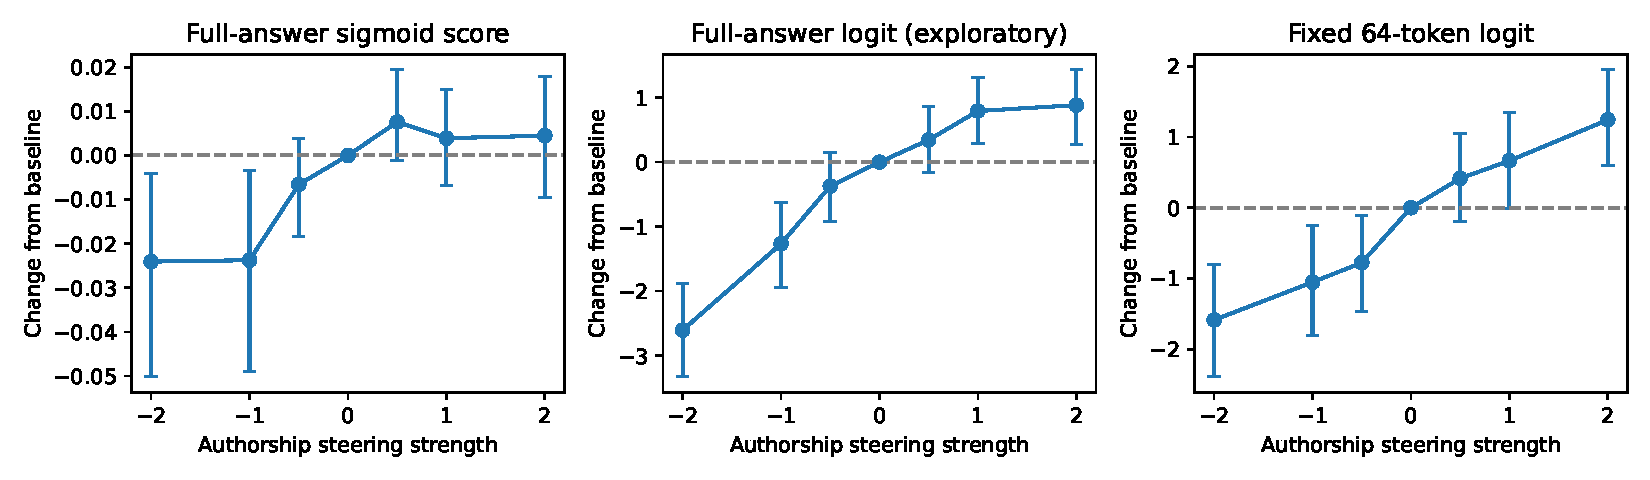
\includegraphics[width=\textwidth]{figures/modern_dose.pdf}
\caption{Exploratory Desklib outcomes. Sigmoid scores are near ceiling, so logit changes are more visible than probability-scale changes. Fixed-prefix eligibility is treatment-dependent. Logit analysis was added after inspecting saturation and is not a prespecified primary endpoint.}
\label{fig:modern}
\end{figure*}

We separately stress-tested the quality rubric on 20 baseline answers and 60 constructed corruptions, with unchanged blinded prompts. Mean coherence falls from 4.40 to 2.60 under word shuffling and to 1.60 under repetition; adequacy falls from 4.75 to 1.00 when an unrelated answer is substituted. Thus the rubric detects clear failures, even though its AI-style score does not track provenance. This audit validates sensitivity to gross corruption, not factual accuracy or subtle semantic preservation.
